%============================================================================%
% Antoine Gé́ré (gereantoine@gmail.com). 
%============================================================================%                                                     

%-- CLASS ------------------------------------------------------------------%

\documentclass[9pt]{beamer} 

\pdfoutput=1 

\makeatletter 

%-- PACKAGES ----------------------------------------------------------------%

\usepackage{amscd}
\usepackage{amsmath}
\usepackage{amsthm}
\usepackage{amsxtra}
\usepackage{array} 

\usepackage[english]{babel} 

\usepackage{cancel}
\usepackage{color}

\usepackage{enumitem}

\usepackage{fancyhdr}
\usepackage[T1]{fontenc} 

\usepackage{geometry} 
\usepackage{graphicx} 

\usepackage{hyperref} 

\usepackage[utf8]{inputenc} 

\usepackage{letltxmacro}
\usepackage{lmodern}

\usepackage{manfnt}
\usepackage{multicol} 

\usepackage[numbers,sort]{natbib}

\usepackage{pgf}

\usepackage{setspace} 

\usepackage{tikz}

\usepackage{url}
 
\usepackage{wasysym}
\usepackage{wrapfig}

\usepackage{xcolor}

%-- THEME -------------------------------------------------------------------%

\mode<presentation>
{

  %== NAVIGATION SYMBOLS ======================================================%    

  \setbeamertemplate{navigation symbols}{}
  
  %== TITLE PAGE ==============================================================%    

  \newcommand\coauthor[1]{\def\insertcoauthor{#1}}
  \coauthor{}

  \newcommand\conference[1]{\def\insertconference{#1}}
  \conference{}

  \newcommand\shortconference[1]{\def\insertshortconference{#1}}
  \shortconference{}

  \newcommand\paper[1]{\def\insertpaper{#1}}
  \paper{}

  \newcommand\LogoUniv[1]{\def\insertLogoUniv{#1}}
  \paper{}
  
  \newcommand\TitlePic[1]{\def\insertTitlePic{#1}}
  \paper{}

  \pgfdeclareverticalshading[title page.bg]{beamer@titleshade}{\paperwidth}{%
    color(0pt)=(black!30!white);
    color(3pt)=(black!60!white);
    color(3pt)=(title page.bg);
    color(113pt)=(title page.bg);
    color(113pt)=(black!60!white);
    color(116pt)=(black!30!white)}
  
  \defbeamertemplate*{title page}{gottingen14}[1][]
  {%
    \hbox{%
      %
      \leavevmode%
      \advance\beamer@leftmargin by -12bp%
      \advance\beamer@rightmargin by -12bp%
      \beamer@tempdim=\textwidth%
      \advance\beamer@tempdim by \beamer@leftmargin%
      \advance\beamer@tempdim by \beamer@rightmargin%
      \hskip-\Gm@lmargin%
      %
      \hbox{%
	\setbox%
	\beamer@tempbox=\hbox{%
	%
	\begin{minipage}[b]{\paperwidth}%
	  \vbox{}%
	  \leavevmode%
	  \center{%
	    {\usebeamerfont{title}\inserttitle}\\[5pt]%
	    {\usebeamerfont{author}\color{black}\insertauthor}\\[1pt]%
	    %\insertLogoUniv
	    {\usebeamerfont{institute}\color{black}\insertinstitute}\\[-2pt]%
	    {\usebeamerfont{conference}\color{black}\insertconference, \insertdate}\\[1pt]%
	    {\usebeamerfont{coauthor}\color{black} joint work with \insertcoauthor}\\[-3pt]%
	    {\usebeamerfont{paper}\color{black}\insertpaper}%
	  }%
	  \strut%
	  \par%
	  \vbox{}%
	\end{minipage}%
	}%
	%
	\beamer@tempdim=\ht\beamer@tempbox%
	\advance\beamer@tempdim by 125pt%
	%
	\begin{pgfpicture}{0pt}{0pt}{\paperwidth}{\beamer@tempdim}
	  \pgfsetfillopacity{0.8}
	  \pgftext[left,base]{\pgfuseshading{beamer@titleshade}}
	\end{pgfpicture}
	%
	\hskip-\paperwidth%
	\box\beamer@tempbox%
      }%
    }%
  }

  %== TEMPLATE ================================================================% 
 
  \setbeamertemplate{title page}[gottingen14][colsep=-4bp,rounded=false]
  \setbeamertemplate{sections/subsections in toc}[ball]
  \setbeamertemplate{items}[ball]
  \setbeamertemplate{blocks}[default]
  \setbeamertemplate{part page}[default][colsep=-4bp,rounded=false]
    
  %== COLOR ===================================================================% 
  
  \setbeamercolor{title page}{bg=white!96!black,fg=red!62!black}
  \setbeamercolor{frametitle}{bg=white,fg=red!60!black}
  \setbeamercolor{subsection in head/foot}{bg=white!95!black,fg=red!60!black}
  \setbeamercolor{author in head/foot}{bg=white,fg=red!60!black}
  \setbeamercolor{title in head/foot}{bg=white,fg=red!60!black}
  \setbeamercolor{normal text}{black}
  \setbeamercolor{headline@color}{bg=black,fg=green}
  \setbeamercolor{block title}{bg=black!20!white,fg=white}
  \setbeamercolor{block body}{bg=black!20!white,fg=black}
  \setbeamercolor{block body alerted}{bg=black!40!white,fg=black}
  \setbeamercolor{block title alerted}{bg=black!40!white,fg=black}
  \setbeamercolor{block body example}{bg=black!10!white,fg=black}
  \setbeamercolor{block title example}{bg=black!10!white,fg=black}
  \setbeamercolor{button}{bg=black!50!white,fg=white}
  \setbeamercolor{sidebar}{bg=black,fg=white}
  \setbeamercolor{palette sidebar primary}{bg=black,fg=white}
  \setbeamercolor{palette sidebar secondary}{bg=black,fg=white}
  \setbeamercolor{palette sidebar tertiary}{bg=black,fg=white}
  \setbeamercolor{palette sidebar quaternary}{bg=black,fg=white}
  \setbeamercolor{titlelike}{bg=green,fg=white}
  \setbeamercolor{separation line}{white}
  \setbeamercolor{fine separation line}{white}

  %== FONT ====================================================================% 
  
  \setbeamerfont{frametitle}{size={\normalsize},series={\bf}}
  \setbeamerfont{block title}{size={\scriptsize},series={}}
  \setbeamerfont{block body}{size={},series={}}
  \setbeamerfont{block title example}{size={\normalsize},series={}}
  \setbeamerfont{block body example}{size={},series={}}
  \setbeamerfont{title}{size={\LARGE},series={\bf}}
  \setbeamerfont{author}{size={\Large},series={\bf}}
  \setbeamerfont{institute}{size={\normalsize},series={}}
  \setbeamerfont{conference}{size={\large},series={}}
  \setbeamerfont{date}{size={\normalsize},series={}}
  \setbeamerfont{coauthor}{size={\normalsize},series={\bf}}
  \setbeamerfont{paper}{size={\normalsize},series={\tt}}

  %== COVERED =================================================================% 
  
  \setbeamercovered{transparent}
    
  %== SHADOWS =================================================================% 

  \AtBeginDocument{%
    \pgfdeclareverticalshading{beamer@topshade}{\paperwidth}{%
      color(0pt)=(bg);%
      color(4pt)=(black!50!bg)}%
    \pgfdeclareverticalshading{beamer@bottomshade}{\paperwidth}{%
      color(0pt)=(black!50!bg);%
      color(4pt)=(bg)}%
    \pgfdeclarehorizontalshading{beamer@rightshade}{\paperwidth}{%
      color(0pt)=(black!50!bg);%
      color(4pt)=(bg)}%
    \pgfdeclarehorizontalshading{beamer@leftshade}{\paperwidth}{%
      color(0pt)=(black!50!bg);%
      color(4pt)=(bg)}%
  }%

  %== FRAME TITLE =============================================================% 

    \pgfdeclareverticalshading[frametitle.bg]{beamer@frametitleshade}{\paperwidth}
    {%
      color(0pt)=(frametitle.bg);
      color(36pt)=(frametitle.bg)
    }%

    \defbeamertemplate*{frametitle}{nosplit theme}
    {%
      \nointerlineskip%
      \vskip-2.5pt%
      \hbox{\leavevmode
        \advance\beamer@leftmargin by -12bp%
        \advance\beamer@rightmargin by -12bp%
        \beamer@tempdim=\textwidth%
        \advance\beamer@tempdim by \beamer@leftmargin%
        \advance\beamer@tempdim by \beamer@rightmargin%
        \hskip-\Gm@lmargin\hbox{%
          \setbox\beamer@tempbox=\hbox{
          \begin{minipage}[b]{\paperwidth}%
              \vbox{}%
              \vskip0ex%
              \leftskip0.3cm%
              \rightskip0.3cm plus1fil\leavevmode
              \insertframetitle%
              \ifx\insertframesubtitle\@empty%
                \strut\par%
              \else
                \par{\usebeamerfont*{framesubtitle}{\insertframesubtitle}\strut\par}%
              \fi%
              \vskip5pt%
              \nointerlineskip
              \vbox{}%
              \end{minipage}}%
          \beamer@tempdim=\ht\beamer@tempbox%
          \advance\beamer@tempdim by 2pt%
          \begin{pgfpicture}{0pt}{0pt}{\paperwidth}{\beamer@tempdim}
            \usebeamercolor{frametitle}
            \pgfpathrectangle{\pgfpointorigin}{\pgfpoint{\paperwidth}{\beamer@tempdim}}
            \pgfusepath{clip}
            \pgftext[left,base]{\pgfuseshading{beamer@frametitleshade}}
          \end{pgfpicture}
          \hskip-\paperwidth%
          \box\beamer@tempbox%
        }%
        \hskip-\Gm@rmargin%
      }%
      \nointerlineskip
        \vskip-0.2pt
        \hbox to\textwidth{\hskip-\Gm@lmargin\pgfuseshading{beamer@topshade}\hskip-\Gm@rmargin}
        \vskip-2pt
    }

  %== FOOTLINE ================================================================%    

  \newcommand{\backupbegin}{
    \newcounter{framenumberappendix}
    \setcounter{framenumberappendix}{\value{framenumber}}
  }

  \newcommand{\backupend}{
    \addtocounter{framenumberappendix}{-\value{framenumber}}
    \addtocounter{framenumber}{\value{framenumberappendix}} 
  }

  \defbeamertemplate*{footline}{nosplit theme}{%
    \vskip1pt
    \pgfuseshading{beamer@bottomshade}
    \vskip1.5pt
    \leavevmode%
    \hbox{%
      \begin{beamercolorbox}[wd=.2\paperwidth,center]{footline@color}%
	\usebeamerfont{author in head/foot} \insertauthor
      \end{beamercolorbox}%
      \begin{beamercolorbox}[wd=.2\paperwidth,center]{footline@color}%
	\usebeamerfont{institute in head/foot} \insertshortconference
      \end{beamercolorbox}%
      \begin{beamercolorbox}[wd=.5\paperwidth,center]{footline@color}%
	\usebeamerfont{title in head/foot} \inserttitle 
      \end{beamercolorbox}%
      \begin{beamercolorbox}[wd=.1\paperwidth,center]{footline@color}%
	\insertframenumber{} / \inserttotalframenumber 
      \end{beamercolorbox}%
    }%
    \vskip0.5pt%
  }%
%
}%
%
\mode%
%
<all>

%-- COMMANDS ----------------------------------------------------------------%

\newcommand{\bra}[1]{\langle{#1}|} % Define the Bra.       
\newcommand{\ket}[1]{|{#1}\rangle} % Define the Ket.

\newcommand{\Bracket}[2]{\langle #1 | #2 \rangle} % Define the bracket
\newcommand{\PB}[1]{\left\{{#1}\right\}} % Define the Poisson bracket.
\newcommand{\Comut}[1]{\left[ #1 \right]} % Define the commutator.

\newcommand{\Tdot}{\cdot_\Tsf} % Define the symbol for the general time ordering product.
\newcommand{\TdotH}{\cdot_{\Tsf_\Hsf}} % Define the symbol for the time ordering product defined for H.

\newcommand{\Smearip}[1]{\left\langle #1 \right\rangle} % Define the smearing product.

\newcommand{\abs}[1]{\left|{#1}\right|} % Define the absolute value.
\newcommand{\norm}[1]{\left|{#1}\right|} % Definie the norm.
\newcommand{\dmu}[1]{\dsf\mu_{#1}} % Definie the symbol for the measure.

\newcommand{\expo}{\mathsf{exp}} % Define the exponential exp.
\newcommand{\E}{\mathsf{e}} % Define the exponential e.
\newcommand{\logar}{\mathsf{log}} % Define the logarithm.
\renewcommand{\sin}{\mathsf{sin}} % Redefine the sinus.
\renewcommand{\cos}{\mathsf{cos}} % Redefine the cosinus.
\renewcommand{\tan}{\mathsf{tan}} % Redefine the tangent.
\renewcommand{\arcsin}{\mathsf{arcsin}} % Redefine the arcsinus.
\renewcommand{\arccos}{\mathsf{arccos}} % Redefine the arccosinus.
\renewcommand{\arctan}{\mathsf{arctan}} % Redefine the arctangent.

\renewcommand{\inf}{\mathsf{inf}} % Redefine the inf.
\renewcommand{\sup}{\mathsf{sup}} % Redefine the sup.
\renewcommand{\deg}{\mathsf{deg}} % Redefine the degree of a polynom.

\renewcommand{\arg}{\mathsf{arg}} % Redefine the argument.
\newcommand{\Arg}{\mathsf{Arg}} % Redefine the principal value of the\cite[p.646]{BF2000} argument.

\renewcommand{\Re}{\mathsf{Re}} % Define the real part.
\renewcommand{\Im}{\mathsf{Im}} % Define the imaginary part.

\newcommand{\pp}{\mathsf{pp}} % Define the principal part.
\newcommand{\rp}{\mathsf{rp}} % Define the regular part.

\newcommand{\pv}{\mathsf{pv}} % Define the principal value.

\renewcommand{\det}{\mathsf{det}} % Redefine the determinant.
\newcommand{\tr}{\mathsf{Tr}} % Define the trace.

\newcommand{\cg}[6]{\left(\begin{array}{cc|c} #1 & #3 & #5 \\ #2 & #4 & #6 \end{array}\right)} % Define the symbole for Clebsch Gordan coefficients.
\newcommand{\wig}[6]{\left(\begin{array}{ccc} #1 & #3 & #5 \\ #2 & #4 & #6 \end{array}\right)} % Define the symbole for the 3-j (Wigner symbols).

\newcommand{\wick}[1]{:\!{#1}\!:} % Define the wick product.

\newcommand{\WF}{\mathsf{WF}} % Define the wave front set.
\newcommand{\supp}{\mathsf{supp}} % Define the support.
\newcommand{\Smatrix}{\mathbf{\mathsf{S}}}% Define the S matrix.

\newcommand{\sd}{\mathsf{sd}} % Define the scaling degree.
\renewcommand{\div}{\mathsf{div}} % Redefine the divergence degree.

\newcommand{\EndDfn}{\hfill\ensuremath{\blacktriangleright}} % Define the symbol for the end of definitions.
\newcommand{\EndLem}{\hfill\ensuremath{\rhd}} % Define the symbol for the end of lemmas.
\newcommand{\EndThm}{\hfill\ensuremath{\rhd}} % Define the symbol for the end of theorems.
\newcommand{\EndDemo}{\hfill\ensuremath{\blacksquare}} % Define the symbol for the end of proofs.
\newcommand{\EndEx}{\hfill\ensuremath{\circ}} % Define the symbol for the end of examples.
\newcommand{\EndAxiom}{\hfill\ensuremath{\bullet}} % Define the symbol for the end of list of axioms.
\newcommand{\EndCorol}{\hfill\ensuremath{\rhd}} % Define the symbol for the end of corollaries.
\newcommand{\EndProp}{\hfill\ensuremath{\rhd}} % Define the symbol for the end of properties.

\newcommand{\diff}[2]{\frac{\mathrm{d}#1}{\mathrm{d}#2}} % Define the derivatives.
\newcommand{\partdiff}[2]{\frac{\partial#1}{\partial#2}} %  Define the partial derivatives.

\newcommand{\Retsol}{\Gsf_{\mathsf{r}}} % Define the retarded fundamental solution.
\newcommand{\Advsol}{\Gsf_{\mathsf{a}}} % Define the advanced fundamental solution.
\newcommand{\DisDelta}{\mathsf{\Delta}} % Define the symbol to the the bidistribution associated to the causal propagator.

\newcommand{\CoLine}{\oslash} % Define the symbol for the line complement.
\newcommand{\CoVertex}{\odot} % Define the symbol for the vertex complement.
\newcommand{\Part}{\mathsf{Part}} % Define the symbol for the partition.

\newcommand{\lc}{\Vcal} % Define the symbol for the light cone.

\newcommand{\citebeam}[1]{\textit{\textcolor{black!60!white}{[#1]}}} % Define cite for beamer

\newcommand*\circled[1]{\tikz[baseline=(char.base)]{\node[shape=circle,draw,inner sep=2pt] (char) {#1};}} % Define circled numbers.

%-- ALPHABET IN mathcal MODE ------------------------------------------------%

\newcommand{\Acal}{\mathcal{A}}
\newcommand{\Bcal}{\mathcal{B}}
\newcommand{\Ccal}{\mathcal{C}}
\newcommand{\Dcal}{\mathcal{D}}
\newcommand{\Ecal}{\mathcal{E}}
\newcommand{\Fcal}{\mathcal{F}}
\newcommand{\Gcal}{\mathcal{G}}
\newcommand{\Hcal}{\mathcal{H}}
\newcommand{\Ical}{\mathcal{I}}
\newcommand{\Jcal}{\mathcal{J}}
\newcommand{\Kcal}{\mathcal{K}}
\newcommand{\Lcal}{\mathcal{L}}
\newcommand{\Mcal}{\mathcal{M}}
\newcommand{\Ncal}{\mathcal{N}}
\newcommand{\Ocal}{\mathcal{O}}
\newcommand{\Pcal}{\mathcal{P}}
\newcommand{\Qcal}{\mathcal{Q}}
\newcommand{\Rcal}{\mathcal{R}}
\newcommand{\Scal}{\mathcal{S}}
\newcommand{\Tcal}{\mathcal{T}}
\newcommand{\Ucal}{\mathcal{U}}
\newcommand{\Vcal}{\mathcal{V}}
\newcommand{\Wcal}{\mathcal{W}}
\newcommand{\Xcal}{\mathcal{X}}
\newcommand{\Ycal}{\mathcal{Y}}
\newcommand{\Zcal}{\mathcal{Z}}

%-- ALPHABET IN mathbb MODE ------------------------------------------------%

\newcommand{\Abb}{\mathbb{A}}
\newcommand{\Bmbb}{\mathbb{B}}
\newcommand{\Cbb}{\mathbb{C}}
\newcommand{\Dbb}{\mathbb{D}}
\newcommand{\Ebb}{\mathbb{E}}
\newcommand{\Fbb}{\mathbb{F}}
\newcommand{\Gbb}{\mathbb{G}}
\newcommand{\Hbb}{\mathbb{H}}
\newcommand{\Ibb}{\mathbb{I}}
\newcommand{\Jbb}{\mathbb{J}}
\newcommand{\Kbb}{\mathbb{K}}
\newcommand{\Lbb}{\mathbb{L}}
\newcommand{\Mbb}{\mathbb{M}}
\newcommand{\Nbb}{\mathbb{N}}
\newcommand{\Obb}{\mathbb{O}}
\newcommand{\Pbb}{\mathbb{P}}
\newcommand{\Qbb}{\mathbb{Q}}
\newcommand{\Rbb}{\mathbb{R}}
\newcommand{\Sbb}{\mathbb{S}}
\newcommand{\Tbb}{\mathbb{T}}
\newcommand{\Ubb}{\mathbb{U}}
\newcommand{\Vbb}{\mathbb{V}}
\newcommand{\Wbb}{\mathbb{W}}
\newcommand{\Xbb}{\mathbb{X}}
\newcommand{\Ybb}{\mathbb{Y}}
\newcommand{\Zbb}{\mathbb{Z}}

%-- ALPHABET IN mathfrak MODE ----------------------------------------------%

\newcommand{\Arak}{\mathfrak{A}}
\newcommand{\Brak}{\mathfrak{B}}
\newcommand{\Crak}{\mathfrak{C}}
\newcommand{\Drak}{\mathfrak{D}}
\newcommand{\Erak}{\mathfrak{E}}
\newcommand{\Frak}{\mathfrak{F}}
\newcommand{\Grak}{\mathfrak{G}}
\newcommand{\Hrak}{\mathfrak{H}}
\newcommand{\Irak}{\mathfrak{I}}
\newcommand{\Jrak}{\mathfrak{J}}
\newcommand{\Krak}{\mathfrak{K}}
\newcommand{\Lrak}{\mathfrak{L}}
\newcommand{\Mrak}{\mathfrak{M}}
\newcommand{\Nrak}{\mathfrak{N}}
\newcommand{\Orak}{\mathfrak{O}}
\newcommand{\Prak}{\mathfrak{P}}
\newcommand{\Qrak}{\mathfrak{Q}}
\newcommand{\Rrak}{\mathfrak{R}}
\newcommand{\Srak}{\mathfrak{S}}
\newcommand{\Trak}{\mathfrak{T}}
\newcommand{\Urak}{\mathfrak{U}}
\newcommand{\Vrak}{\mathfrak{V}}
\newcommand{\Wrak}{\mathfrak{W}}
\newcommand{\Xrak}{\mathfrak{X}}
\newcommand{\Yrak}{\mathfrak{Y}}
\newcommand{\Zrak}{\mathfrak{Z}}

%-- ALPHABET IN mathsf MODE ----------------------------------------------%

\newcommand{\Asf}{\mathsf{A}}
\newcommand{\Bsf}{\mathsf{B}}
\newcommand{\Csf}{\mathsf{C}}
\newcommand{\Dsf}{\mathsf{D}}
\newcommand{\Esf}{\mathsf{E}}
\newcommand{\Fsf}{\mathsf{F}}
\newcommand{\Gsf}{\mathsf{G}}
\newcommand{\Hsf}{\mathsf{H}}
\newcommand{\Isf}{\mathsf{I}}
\newcommand{\Jsf}{\mathsf{J}}
\newcommand{\Ksf}{\mathsf{K}}
\newcommand{\Lsf}{\mathsf{L}}
\newcommand{\Msf}{\mathsf{M}}
\newcommand{\Nsf}{\mathsf{N}}
\newcommand{\Osf}{\mathsf{O}}
\newcommand{\Psf}{\mathsf{P}}
\newcommand{\Qsf}{\mathsf{Q}}
\newcommand{\Rsf}{\mathsf{R}}
\newcommand{\Ssf}{\mathsf{S}}
\newcommand{\Tsf}{\mathsf{T}}
\newcommand{\Usf}{\mathsf{U}}
\newcommand{\Vsf}{\mathsf{V}}
\newcommand{\Wsf}{\mathsf{W}}
\newcommand{\Xsf}{\mathsf{X}}
\newcommand{\Ysf}{\mathsf{Y}}
\newcommand{\Zsf}{\mathsf{Z}}

\newcommand{\asf}{\mathsf{a}}
\newcommand{\bsf}{\mathsf{b}}
\newcommand{\csf}{\mathsf{c}}
\newcommand{\dsf}{\mathsf{d}}
\newcommand{\esf}{\mathsf{e}}
\newcommand{\fsf}{\mathsf{f}}
\newcommand{\gsf}{\mathsf{g}}
\newcommand{\hsf}{\mathsf{h}}
\newcommand{\isf}{\mathsf{i}}
\newcommand{\jsf}{\mathsf{j}}
\newcommand{\ksf}{\mathsf{k}}
\newcommand{\lsf}{\mathsf{l}}
\newcommand{\msf}{\mathsf{m}}
\newcommand{\nsf}{\mathsf{n}}
\newcommand{\osf}{\mathsf{o}}
\newcommand{\psf}{\mathsf{p}}
\newcommand{\qsf}{\mathsf{q}}
\newcommand{\rsf}{\mathsf{r}}
\newcommand{\ssf}{\mathsf{s}}
\newcommand{\tsf}{\mathsf{t}}
\newcommand{\usf}{\mathsf{u}}
\newcommand{\vsf}{\mathsf{v}}
\newcommand{\wsf}{\mathsf{w}}
\newcommand{\xsf}{\mathsf{x}}
\newcommand{\ysf}{\mathsf{y}}
\newcommand{\zsf}{\mathsf{z}}

%-- ALPHABET IN mathbf MODE ----------------------------------------------%

\newcommand{\Abf}{\mathbf{A}}
\newcommand{\Bbf}{\mathbf{B}}
\newcommand{\Cbf}{\mathbf{C}}
\newcommand{\Dbf}{\mathbf{D}}
\newcommand{\Ebf}{\mathbf{E}}
\newcommand{\Fbf}{\mathbf{F}}
\newcommand{\Gbf}{\mathbf{G}}
\newcommand{\Hbf}{\mathbf{H}}
\newcommand{\Ibf}{\mathbf{I}}
\newcommand{\Jbf}{\mathbf{J}}
\newcommand{\Kbf}{\mathbf{K}}
\newcommand{\Lbf}{\mathbf{L}}
\newcommand{\Mbf}{\mathbf{M}}
\newcommand{\Nbf}{\mathbf{N}}
\newcommand{\Obf}{\mathbf{O}}
\newcommand{\Pbf}{\mathbf{P}}
\newcommand{\Qbf}{\mathbf{Q}}
\newcommand{\Rbf}{\mathbf{R}}
\newcommand{\Sbf}{\mathbf{S}}
\newcommand{\Tbf}{\mathbf{T}}
\newcommand{\Ubf}{\mathbf{U}}
\newcommand{\Vbf}{\mathbf{V}}
\newcommand{\Wbf}{\mathbf{W}}
\newcommand{\Xbf}{\mathbf{X}}
\newcommand{\Ybf}{\mathbf{Y}}
\newcommand{\Zbf}{\mathbf{Z}}

\newcommand{\abf}{\mathbf{a}}
\newcommand{\bbf}{\mathbf{b}}
\newcommand{\cbf}{\mathbf{c}}
\newcommand{\dbf}{\mathbf{d}}
\newcommand{\ebf}{\mathbf{e}}
\newcommand{\fbf}{\mathbf{f}}
\newcommand{\gbf}{\mathbf{g}}
\newcommand{\hbf}{\mathbf{h}}
\newcommand{\ibf}{\mathbf{i}}
\newcommand{\jbf}{\mathbf{j}}
\newcommand{\kbf}{\mathbf{k}}
\newcommand{\lbf}{\mathbf{l}}
\newcommand{\mbf}{\mathbf{m}}
\newcommand{\nbf}{\mathbf{n}}
\newcommand{\obf}{\mathbf{o}}
\newcommand{\pbf}{\mathbf{p}}
\newcommand{\qbf}{\mathbf{q}}
\newcommand{\rbf}{\mathbf{r}}
\newcommand{\sbf}{\mathbf{s}}
\newcommand{\tbf}{\mathbf{t}}
\newcommand{\ubf}{\mathbf{u}}
\newcommand{\vbf}{\mathbf{v}}
\newcommand{\wbf}{\mathbf{w}}
\newcommand{\xbf}{\mathbf{x}}
\newcommand{\ybf}{\mathbf{y}}
\newcommand{\zbf}{\mathbf{z}}

%-- THEOREM ENVIRONMENTS ---------------------------------------------------------%

\newtheorem{thm}{Theorem}
\newtheorem{lem}{Lemma}
\newtheorem{prop}{Proposition}
\newtheorem{corol}{Corollary}
\newtheorem{demo}{Proof}
\newtheorem{axiom}{Axiom}
\newtheorem{axioms}{Axioms}

\newtheorem{dfn}{Definition}
\newtheorem{dfns}{Definitions}
\newtheorem{rmk}{Remark}
\newtheorem{rmks}{Remarks}
\newtheorem{ex}{Example}
\newtheorem{exs}{Examples}

%-- LIST SETTINGS ----------------------------------------------------------------%

\setlist[itemize]{%
  align=left,
  labelsep=*,
  leftmargin=12pt,
  topsep=4pt, 
  itemsep=12pt,
  label=$\bullet$
}

\setlist[description]{
  leftmargin=12pt,
  itemsep=6pt,
  label=$\bullet$
}

\linespread{1.4}

%-- HYPERREF ----------------------------------------------------------------%

%\definecolor{darkcerulean}{rgb}{0.03, 0.27, 0.49}

\hypersetup{     
 unicode=false,      
 pdftoolbar=true,    
 pdfmenubar=true,    
 pdffitwindow=true,  
 pdfstartview={FitH},
 pdftitle={lqp35-antoine},    
 pdfauthor={Antoine Géré},     
 pdfsubject={Mathematical Physics},   
 pdfcreator={LaTeX},  
 pdfproducer={pdfTex},
 pdfkeywords={pertubative algebraic quantum qield Theory, dimensional regularisation.},  
 pdfnewwindow=true,  
 citecolor=darkcerulean,
}

%-- TIKZ LIBRARY ------------------------------------------------------------%

\usetikzlibrary{decorations.pathmorphing,decorations.markings}


%-- TITLE PAGE --------------------------------------------------------------%

\title{Dimensional regularisation on curved spacetime}

\author{\href{mailto:gere@dima.unige.it}{Antoine Géré}}

\coauthor{\href{mailto:hack@dima.unige.it}{Thomas-Paul Hack} and \href{mailto:pinamont@dima.unige.it}{Nicola Pinamonti}}

\date{November 15th, 2014}

\institute{\href{http://www.unige.it/strutture/ou/staff/DIMA}{Università degli studi di Genova, Dipartimento di Matematica}}

\conference{\href{http://www.uni-math.gwdg.de/bahns/lqp35/}{LQP 35th, Goslar}}

\shortconference{\href{http://www.uni-math.gwdg.de/bahns/lqp35/}{LQP 35th}}

\paper{\href{http://arxiv.org/}{to appear soon on arXiv}}

%============================================================================%
\begin{document}
%============================================================================%

\selectlanguage{english}

%----------------------------------------------------------------------------%

{ 
  \setbeamertemplate{footline}{} 
  \setbeamertemplate{headline}{}
  \setbeamertemplate{background}{\includegraphics[width=\paperwidth,height=\paperheight]{fig_balbi}}
  \begin{frame}[plain]
    \titlepage
  \end{frame}
}

%----------------------------------------------------------------------------%
\section{Intro.} 
%----------------------------------------------------------------------------%

\begin{frame}

  \frametitle{Motivation}
  
  \begin{itemize}
    
    \item pertubative algebraic quantum field theory (pAQFT) \\
    $\to$ \textbf{conceptually well known} \\
    \citebeam{Brunetti, Dütsch, Fredenhagen, Hollands, K\"ohler, Rejzner, Wald, ... $\sim$1996-2013} \\
    
    \item in pAQFT on curved spacetime (CST), regularisation uses ideas of Epstein and Glaser \\
    $\to$ procedure \textbf{unconvenient for computations} \\
    \citebeam{Brunetti \& Fredenhagen 2000, Hollands \& Wald 2002, Dang 2013} \\
    
    \item desire to use framework of pAQFT for \textbf{cosmological model}! \\
    %\citebeam{Dappiaggi, Moretti, Pinamonti 2009, Hack 2010}
  
  \end{itemize}

\end{frame}

%----------------------------------------------------------------------------%

\begin{frame}

  \frametitle{What I am going to talk about}
  
  \begin{itemize}
   
    \item \textbf{pAQFT} $\to$ in order to identify the regularisation problem! \\
   
    \item a framework for a \textbf{dimensional regularisation} on CST \\
    $\to$ a general procedure more computationally friendly! \\
   
    \item explicit computations on spatially flat Friedmann Lemaître Robertson Walker spacetimes \\
    $\to$ finally a \textbf{bit of practice}!
   
  \end{itemize}

\end{frame}

%----------------------------------------------------------------------------%
\section{pAQFT}
%----------------------------------------------------------------------------%

{
\setbeamertemplate{footline}{} 
\setbeamertemplate{headline}{}
\setbeamertemplate{background}{\includegraphics[width=\paperwidth,height=\paperheight]{fig_paqft}}
\pgfsetfillopacity{0.8}
\begin{frame}
\bf
\vspace*{30pt}
\begin{exampleblock}{\vspace*{-3ex}}
\begin{center}
\Large Pertubative Algebraic Quantum Field Theory \\[10pt] on Curved Spacetime
\end{center}
\end{exampleblock}
\end{frame}
}

%----------------------------------------------------------------------------%

\begin{frame}

  \frametitle{Functional Approach}
  
  \begin{itemize}
  
    \item $(\Mcal,\gsf)$ : \textbf{4 dimensional} globally hyperbolic spacetime 
    
    \item \textbf{off shell} configuration space $\to$ scalar field $\phi \in \Ccal^\infty(\Mcal,\Rbb)$
        
    \item $\Fcal$: \textbf{space of observables}
    $\ \Fsf : \left\{
     \begin{array}{ccc}
       \Ccal^\infty(\Mcal,\Rbb) & \to & \Cbb \\
       \phi & \mapsto & \Fsf(\phi)
     \end{array}
     \right.
    $
   
   \vspace*{10pt}
   
   \textbf{Spacetime support} of $\Fsf$
    \begin{equation*}
      \supp(\Fsf) \doteq \left\{ x \in \Mcal \bigg| 
      \begin{array}{l} 
	\forall \ \mbox{neighborhood } U \mbox{ of } x, \ \exists \ \phi, \psi \in \mbox{ smooth}, \\
	\supp(\psi) \subset U, \mbox{ such that } \Fsf(\phi + \psi) \neq \Fsf(\phi).
      \end{array}
      \right\}
   \end{equation*}
   
% \vspace*{-2pt}
 

 
  %\vspace*{15pt}
   
  %\begin{alertblock}{} 
    %\vspace*{-16pt}
    %\begin{center}
     % \begin{tabular}{ccc}
	%configuration $\phi$ & : & pure state in classical field theory \\[3pt]
	%functional $\Fsf$ & : & observable \\[3pt]
	%$\Fsf(\phi)$ & : & outcome of the measurement of $\Fsf$ in $\phi$
     % \end{tabular}
    %\end{center}
   % \vspace*{-12pt}
  %\end{alertblock}

  \end{itemize}
 
  
\end{frame}

%----------------------------------------------------------------------------%

\begin{frame}[label=wf]

  \frametitle{Spaces of Observables}

\hfill \hyperlink{details_wf}{\beamergotobutton{wave front set}}

\vspace*{-10pt}

\begin{itemize}
 
 
 \item \textbf{Regular} functionals $\Fcal_{\mathsf{reg}}$ \\[-12pt]   
    \begin{equation*}
      \Fcal_{\mathsf{reg}} = \left\{ \Fsf \ | \ \Fsf \mbox{ smooth}, \Fsf^{(n)} \mbox{ comp. sup.}, \mbox{ and } \WF(\Fsf^{(n)}) = \emptyset \right\} 
    \end{equation*}
    

  
  \item \textbf{Microcausal} functionals $\Fcal_{\mu\csf}$ \\[-24pt]    
  \begin{equation*}
    \Fcal_{\mu\csf} = \left\{ \Fsf \ | \ \Fsf \mbox{ smooth}, \Fsf^{(n)} \mbox{comp. sup.}, \WF(\Fsf^{(n)}) \cap \left( \Mcal^n \times ( \overline{V^{n}_{+}} \cup \overline{V^{n}_{-}} ) \right)  = \emptyset \right\} 
    \vspace*{-8pt}
  \end{equation*}
  \hspace*{15pt} $\to$ local interactions are a subset $\Fcal_{\mathsf{loc}} \subset \Fcal_{\mu\csf}$ 
  
  \vspace*{14pt}
  
  %\item 
  \hspace*{2pt}% 
  \textbf{Interactions} $\to$ \textbf{Local} functionals $\Fcal_{\mathsf{loc}}$ \\[-12pt]
  \begin{equation*}
    \Fcal_{\mathsf{loc}} = \left\{ \Fsf \in \Fcal_{\mu\csf} \ | \ \supp(\Fsf^{(n)}) \subset \{ (x,\dots,x) \subset \Mcal^n \} \right\}
    %\vspace*{-2pt}
  \end{equation*}
  %\hspace*{15pt} 
  \hspace*{2pt}%
  Example: $\Fsf \in \Fcal_\mathsf{loc}(\Mcal)$
  \vspace*{-2pt}
  \begin{equation*}
    \Fsf(\phi) = \int_\Mcal \dsf\mu \ f(x) \ \frac{\lambda}{4!} \phi(x)^4 \ , \ \mbox{with} \ f \in \Ccal^\infty_0(\Mcal,\Rbb)
  \end{equation*}

  \end{itemize}

\end{frame}

%----------------------------------------------------------------------------%

\begin{frame}[label=products]

\frametitle{Poducts of Observables}

\textbf{``Deformation''} of the \textbf{pointwise product} on $\Fcal_\Tsf \subset \Fcal_{\mu\csf}$: \\
$\to$ $\star_\Hsf$ product, defined with $\Hsf_+$ (implement ``quantum structure'') \\
$\to$ $\cdot_\Tsf$ time ordering product, defined with $\Hsf_\fsf$ 
\vspace*{-8pt}
\begin{equation*}
\Fsf \TdotH \Gsf = \Fsf \star_\Hsf \Gsf, \mbox{ if } \supp(\Fsf) \geq \supp(G)
\end{equation*}
\vspace*{-20pt}
\begin{exampleblock}{on a \textbf{normal convex neighborhood} of $x$} 
\vspace*{-18pt}
\begin{eqnarray*}
&& \Hsf_\sharp(x,y) \doteq \lim_{\epsilon \downarrow 0} \ \frac{1}{8\pi^2}\left(\frac{u(x,y)}{\sigma_\sharp(x,y)}+v(x,y)\log(M^2 \sigma_\sharp(x,y))+w(x,y)\right) \\[6pt]
&& \sigma_\pm(x,y) = \sigma(x,y) \pm i\epsilon(t_x-t_y) + \epsilon^2 \qquad \sigma_\fsf(x,y) = \sigma(x,y) + i\epsilon 
\end{eqnarray*}
\vspace*{-14pt}
\end{exampleblock}
\vspace*{-4pt}
$u,v,w:  \mbox{smooth}$, and 2 $\sigma: \mbox{squared geodesic distance}$.
\vspace*{-6pt}


\begin{block}{}
\vspace*{-14pt}
\begin{equation*}
(\Fsf \ \sharp \ \Gsf)(\phi) \ \doteq \ \Fsf(\phi) \cdot \Gsf(\phi) + \sum_{n=1}^{\infty} \frac{\hbar^n}{n!} \Smearip{\Fsf^{(n)},\Hsf_{\sharp}^{\otimes n} \Gsf^{(n)}} \quad \textdbend  
\vspace*{-10pt}
\end{equation*}
%\vspace*{-8pt}
\hfill \hyperlink{details_products}{\beamergotobutton{details}}
\end{block}


\end{frame}

%----------------------------------------------------------------------------%

\begin{frame}
 
\frametitle{Algebra of Observables}

\begin{itemize}
 
\item algebraic structure, with 2 products
\vspace*{-12pt}
\begin{equation*}
\Acal_{\Hsf} = \left( \Fcal_{\Tsf} , \star_\Hsf , \TdotH \right)
\end{equation*}

\item We work with interaction functionals! \\
for $\Fsf \in \Acal_{\Hsf}, \quad
%\vspace*{-12pt}
%\begin{equation*}
\alpha_{\Hsf_+}(\Fsf) = \E^{-\hbar \Gamma_{\Hsf_+}} \Fsf, \quad \mbox{with } \Gamma_{\Hsf_+} = \Smearip{\Hsf_+,\frac{\delta^2}{\delta\phi^2}}  $ \\
%\vspace*{8pt}
%\end{equation*}
e.g. 
$ \alpha_{\Hsf_+}(\phi^2(x)) = \underset{x\to y}{\lim} \left( \phi(x)\phi(y) - \Hsf_+(x,y) \right)$

\item maps of the products \\
for $F, G \in \Fcal_{\Tsf}$, defining $d = \Hsf_+^\prime - \Hsf_+ = \Hsf_\fsf^\prime - \Hsf_\fsf \simeq \frac{1}{8\pi}\left( w^\prime - w \right)$
\vspace*{-4pt}
\begin{eqnarray*}
\Fsf \star_{\Hsf^\prime} \Gsf &=& \alpha_d \left( \alpha_{-d}(\Fsf) \star_\Hsf \alpha_{-d}(\Gsf) \right) \\ 
\Fsf ._{\Tsf_{\Hsf^\prime}} \Gsf &=& \alpha_d \left( \alpha_{-d}(\Fsf) ._{\Tsf_\Hsf} \alpha_{-d}(\Gsf) \right) 
\end{eqnarray*}

\vspace*{-9pt}

\begin{block}{}
\vspace*{-14pt}
\begin{center}
$\Acal_{\Hsf^\prime} \ \sim \ \Acal_{\Hsf}$, the two algebras are isomorphic \\
$\Rightarrow$ thus we will choose a particular representation $\Acal_{\Hsf}$
\end{center}
\vspace*{-5pt}
\end{block}

 


\end{itemize}



\end{frame}

%----------------------------------------------------------------------------%

\begin{frame}%[label=Bogoliubov]

\frametitle{Pertubative picture}

\vspace*{8pt}

$\bullet \quad$ \textbf{Local $\Ssf$ matrix}:
\vspace*{-17pt}
\begin{equation*}
 \hspace*{-25pt} \Ssf(F) = \sum_{n=0}^{\infty} \frac{i^n}{n!} \ \underbrace{\Fsf ._\Tsf \ \dots \ ._\Tsf \Fsf}_{n}
\end{equation*}

\begin{block}{}
\vspace*{-10pt}
\textbf{Microlocal Analysis --  Important property} \citebeam{Hörmander 1983} \\
$u,v \in \Dcal^\prime$, 
\vspace*{-10pt}
\begin{equation*}
%\WF(\Psf u) \subset \WF(u) \ \mbox{ \bf and } \ 
\WF(u) \oplus \WF(v) \not\ni \{0\} \Rightarrow \exists! \ u.v \in \Dcal^\prime
\end{equation*}
\vspace*{-16pt}
\end{block}


$\bullet \quad$ \textbf{Bogoliubov formula} \citebeam{Brunetti, Fredenhagen 2009} \\ %\hfill \hyperlink{details_Bogoliubov}{\beamergotobutton{details}} \\
\vspace*{-10pt}
\begin{equation*}
 \Ssf_\vsf(\Fsf) = \Ssf(\Vsf)^{\star -1} \star \left( \Ssf(\Vsf) ._{\Tsf} \Fsf \right) 
\end{equation*}
$\to$  transition from the free action to the one with additional interaction term $\Vsf$.



\begin{exampleblock}{}
\vspace*{-10pt}
\textbf{Computational trick} \\
for computational convenience, useful to work with $\Acal_{\Delta_+}$ \\
$\to$ $\Delta_+$: the Wightman $2$pt of the free field state $\Omega_0$, $d=\Delta_+ - \Hsf_+$
\end{exampleblock}


  



\end{frame}


%----------------------------------------------------------------------------%
\section{Dim. reg. on CST}
%----------------------------------------------------------------------------%


{
  \setbeamertemplate{footline}{} 
  \setbeamertemplate{headline}{}
  \setbeamertemplate{background}{\includegraphics[width=\paperwidth,height=\paperheight]{fig_dimregcst}}
 \pgfsetfillopacity{0.8}
 \begin{frame}
\bf
 \begin{exampleblock}{\vspace*{-3ex}}
 \begin{center}
 \Large Framework for a Dimensional Regularisation \\[10pt] on Curved Spacetime
 \end{center}
 \end{exampleblock}

\end{frame}
}

%----------------------------------------------------------------------------%
  

\begin{frame}[label=regul_prob]

\frametitle{The regularisation problem}

\textbf{Causality}: \quad $\Fsf ._\Tsf \Gsf = \Fsf \star \Gsf, \mbox{ if } \supp(\Fsf) \geq \supp(G)$ \\
$\to$ %The time ordering is ill defined if $\supp(F) \cap \supp(G) \neq \emptyset$ \\
%\hspace*{10pt} 
$\Hsf_\fsf(x,y)^n$  ill defined if $x=y$ \\[5pt]

\begin{exampleblock}{}
\vspace*{-2ex}
\textbf{Epstein Glaser induction} \citebeam{Brunetti, Fredenhagen 2000} \hfill \hyperlink{proof_EG_induction}{\beamergotobutton{Sketch of the proof}} \\
\textbf{if} $\Fsf_1, \dots, \Fsf_n \in \Fcal_\mathsf{loc}(\Mcal^n)$, \\
\textbf{then} $\Fsf_1 ._\Tsf \ \dots \ \Fsf_n$ can be defined up to $\mathsf{Diag}(\Mcal^n)=\{{\bf x}\in \Mcal^n  | x_1 = \dots = x_n\}$ \\[5pt]
\vspace*{-1ex}
\end{exampleblock}

\textbf{Scaling degree}: For $t \in \Dcal^\prime(\Rbb^4)$ \citebeam{Steinmann 1971} \hfill %\hyperlink{details_scaling_degree}{\beamergotobutton{details}} 
\\[-15pt]
\begin{equation*}
\sd(t) = \inf \{\omega\in\Rbb \ | \ \lim_{\rho \to 0}\rho^\omega t(\rho x)=0 \} 
\end{equation*}

\vspace*{-8pt}

\begin{block}{}
\vspace*{-10pt}
\textbf{``A divergence criterion''}, $t \in \Dcal^\prime(\Rbb^4\backslash\{0\})$ \quad \citebeam{Brunetti, Fredenhagen 2000} \\
$\bullet$ \ \textbf{if} $\sd(t) < 4$, \\
\hspace*{8pt} \textbf{then} $t$ has a unique extension $\dot{t} \in \Dcal^\prime(\Rbb^4)$ with the same scaling degree \\
$\bullet$ \ \textbf{for} $4 \leq \sd(t) < \infty$, $\dot{t}$ has non unique extensions (with same $\sd$)
\end{block}



\end{frame}



%----------------------------------------------------------------------------%

\begin{frame}[label=meromorphic]

\frametitle{Main ideas behind the ``dimensional'' regularisation}



 


\textbf{The reason of our problem}: \\
pointwise powers of $\Delta_\fsf$: ill defined, because contain $\sigma_\fsf^{-n}$ with $n$ too large. \\
Fix $x$ and set the distribution $t(y) = \sigma_\fsf^{-n}(x,y)$, \\
then for $x \to y$, $\sd(t(y)) = 2n$. \\
$\Rightarrow$ $t(y)$ has an unique extension only for $n < 2$

\vspace*{16pt}


\textbf{``Main steps of the recipe''}

(i) Deform $n$ to $n + \alpha$, with $\alpha \in \Cbb$ \\

\qquad \textbf{Result}: the map $\alpha \mapsto \sigma_\fsf^{-(n+\alpha)}$ is meromorphic in $\alpha$. \hfill \hyperlink{proof_meromorphic}{\beamergotobutton{Sketch of the proof}} \\ 
 
(ii) compute the \textbf{Laurent series} with respect to $\alpha$ \\
\qquad $\to$ play with the identities fulfilled by $\sigma$ \\
 
(iii) subtract the principal part \\
 
(iv) take the limit $\alpha \to 0$ \\
 
\end{frame}

%-----------------------------------------------------------------------------%

\begin{frame}[label=fish]

\frametitle{The fish diagram ($2$ vertices)}



\begin{minipage}{0.2\linewidth}
\centering
\begin{figure}
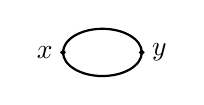
\begin{tikzpicture}[thick,scale=0.5] 
\filldraw (-1,0) circle (1pt) node[left] {$x$};
\filldraw (1,0) circle (1pt) node[right] {$y$};
\draw (0,0) circle (1cm and 0.6cm) ;
\end{tikzpicture}
\end{figure}
\end{minipage}
\hspace*{-8pt}
$\longrightarrow$
\hspace{5pt}
\begin{minipage}{0.7\linewidth}
\vspace*{-4pt}
\begin{equation*}
\Delta_\fsf^2(x,y) = \frac{1}{8 \pi^2} \bigg( \frac{u^2(x,y)}{\sigma_\fsf^2(x,y)} +  
%\underbrace{
\mbox{``well defined for $x=y$''}
%}_{r} 
\bigg)
\end{equation*}
\end{minipage}



\vspace*{20pt}

$\bullet$ regularize only $\sigma_\fsf^{-(2+\alpha)}$ \\

$\bullet$ use $\sigma$ identities : \ $ \Box \sigma = 4 + f \sigma $ \\
 
$\bullet$ $\alpha \mapsto \sigma_\fsf^{-(2+\alpha)}$ (weakly) meromorphic in $\alpha$. \\
\quad $\to$ Laurent series w.r.t $\alpha$ \\
\quad $\to$ subtract the principal part and take the limit $\alpha \to 0$
 
\begin{equation*}
\left(\frac{1}{\sigma_\fsf^2}\right)_\mathsf{reg} \ = \ \lim_{\alpha \to 0} \ \left( 1 - \pp \right) \frac{1}{\sigma_\fsf^{2+\alpha}} 
\end{equation*}
\begin{equation*}
\Longrightarrow \ \left(\Delta_\fsf^{2}\right)_\mathsf{reg} 
\end{equation*}
 
\hfill \hyperlink{details_fish}{\beamergotobutton{details}}

\end{frame}

%----------------------------------------------------------------------------%

\begin{frame}
 
\frametitle{General case (N vertices) I}

\vfill

\begin{wrapfigure}{l}{0.3\textwidth}
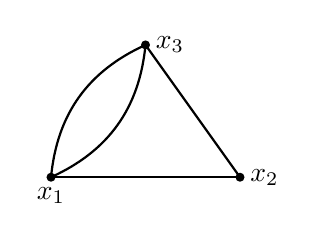
\begin{tikzpicture}[thick,scale=1.2] 
\draw (0,0) -- (2,0);
\draw (2,0) -- (1,1.4);
\draw [bend left] (0,0) edge (1,1.4);
\draw [bend left] (1,1.4) edge (0,0);
\filldraw (0,0) circle (1pt) node[below] {$x_1$};
\filldraw (2,0) circle (1pt) node[right] {$x_2$};
\filldraw (1,1.4) circle (1pt) node[right] {$x_3$};
\end{tikzpicture}
\end{wrapfigure}

$\Gcal$: graph with $N$ vertices $x_1, \dots, x_N$ \\
$x_k$: a reference point arbitrarily chosen
\begin{equation*}
\sigma_{ij} = \sigma_\fsf(x_i,x_j), \quad \sigma_{i} = \sigma_\fsf(x_k,x_j), \quad \sigma^a_{ij} = \nabla^a_i \sigma_{ij}
\end{equation*}

\vfill

\begin{equation*}
\Rightarrow \ t^\alpha(x_1, \dots, x_N) \ = \ \prod_{i<j} \frac{1}{\sigma_{ij}^{n_{ij}+\alpha_{ij}}} , \ \ \alpha_{ij} \in \Cbb
\end{equation*}

$\bullet$ Need a way to isolate the poles in $\{\alpha\}$
\vspace*{-5pt}
\begin{equation*}
\Rsf \doteq \nabla_a^i \sigma_i^a \ \to \ \mbox{``analogue'' of $\Box \sigma + \dots$ that we use in the case $N=2$}
\end{equation*}
\vspace*{-10pt}
\begin{equation*}
\tsf^\alpha \ = \ \frac{1}{\Pcal(N,n_{ij},\alpha_{ij})} \ \left( \Rsf^N \ \tsf^\alpha + \mbox{ ``corr.'' }  \right) 
\end{equation*}

\vfill

\end{frame}

%----------------------------------------------------------------------------%


\begin{frame}
 
\frametitle{General case (N vertices) II}

\begin{itemize}
 
\item then \textbf{apply} $\Rsf$ as many times as \textbf{needed}, to have \textbf{sufficiently small} $\sd$ 

\item the terms in $\logar(\sigma)$ obtained by \textbf{deriving} w.r.t $\alpha_{ij}$

\item subtract the pole \textbf{order by order} as explained or use the \textbf{forest formula} \\
\citebeam{Keller 2010, Dütsch, Fredenhagen, Keller, Rejzner 2013}

\item \textbf{if} $(\Mcal,g)$ has isometries and $\Delta_\fsf$ (i.e. the state $\Omega_0$) is invariant w.r.t. these, \textbf{then} the regularisation scheme preserves this invariance
 
\end{itemize}




\end{frame}

%----------------------------------------------------------------------------%


%\begin{frame}

%\frametitle{A simple diagram with 3 vertices}

%\scriptsize


%\begin{minipage}[b]{0.1\linewidth}
%\centering
%\vspace{pt}
%\begin{tikzpicture}[thick,scale=0.5] 
%\filldraw (0,0) circle (1pt) node[left] {$x_1$};
%\filldraw (1,1) circle (1pt) node[above] {$x_2$};
%\filldraw (2,0) circle (1pt) node[right] {$x_3$};
%\draw (0,0) to[out=0,in=-80] (1,1);
%\draw (0,0) to[out=80,in=170] (1,1);
%\draw (0,0) -- (2,0);
%\draw (1,1) -- (2,0);
%\end{tikzpicture}
%\end{minipage}
%\hspace{8pt}
%\begin{minipage}[b]{0.7\linewidth}
%\vspace*{-4pt}
%\begin{eqnarray*}
 %&& \tsf^\alpha(x_1,x_2,x_3) =  \Delta_\fsf(x_1,x_2)^{2+\alpha_{12}} \ \Delta_\fsf(x_2,x_3)^{1+\alpha_{13}} \ \Delta_\fsf(x_2,x_3)^{1+\alpha_{23}} \\
 %&& \tsf^\alpha
%\end{eqnarray*}
%\end{minipage}




%\end{frame}



%----------------------------------------------------------------------------%
\section{Appli. to FLWR}
%----------------------------------------------------------------------------%


{
  \setbeamertemplate{footline}{} 
  \setbeamertemplate{headline}{}
  \setbeamertemplate{background}{\includegraphics[width=\paperwidth,height=\paperheight]{fig_flwr}}
 
 \pgfsetfillopacity{0.8}
 \begin{frame}
 %\vspace*{120pt}
\bf
 \begin{exampleblock}{\vspace*{-3ex}}
 \begin{center}
 \Large Explicit computations on spatially flat \\[10pt] Friedmann Lemaître Robertson Walker spacetimes
 \end{center}
 \end{exampleblock}

\end{frame}

}

%----------------------------------------------------------------------------%

\begin{frame}
 
\frametitle{Spiatially flat FLWR spacetimes} 
 


\begin{itemize}
 
 
\item \textbf{spatially flat Friedmann Lemaître Robertson Walker} spacetimes
\vspace*{-12pt}
\begin{equation*}
g = a(\tau)^2 \ \left( - d\tau^2 + d\vec{x}^2 \right) 
\vspace*{-8pt}
\end{equation*}

 
\item choosing a \textbf{free field state} $\Omega_0$ (inv. under FLWR sym.) of the quantized free Klein Gordon field on spatially flat FLWR spacetimes \\
$\Delta_\pm$, $\Delta_\fsf$ : can be written using \textbf{spatial Fourier transform} in terms of \textbf{temporal modes} $\chi_k(\tau)$
\vspace*{-6pt}
\begin{equation*}
\left( \partial^2_\tau + k^2 + m^2a^2 + \left( \xi - \frac16 \right)Ra^2 \right) \chi_k(\tau) = 0 
\end{equation*}
\begin{equation*}
\chi_k \partial_\tau \overline{\chi_k} - \overline{\chi_k} \partial_\tau {\chi_k} =i 
\end{equation*}

\item \textbf{in principle} we can compute all quantities in terms of $\vec{k}$- and $\tau$-integrals using our regularisation procedure 
  
\end{itemize}
 
\end{frame}

%----------------------------------------------------------------------------%

\begin{frame}

\frametitle{The conformal trick} 

\begin{itemize}


\item \textdbend \quad Even for spatially flat FLRW spacetimes, \\
$\sigma$, $u$, $v$ are \textbf{not explicitly known} neither in \textbf{position space}, nor in \textbf{$\vec{k}$-space}, \\
$\to$ but we need to know the $\vec{k}$-space version of e.g $\left( \Delta^2_\fsf \right)_\mathsf{reg}$
\vspace*{20pt}

\item \textbf{Trick}: $\Delta_\fsf=\Delta_{\fsf,0}+\delta \Delta_\fsf$, with \\[3pt]

$\to$ $\Delta_{\fsf,0}$ contains sufficiently many singular contributions \\[3pt]

$\to$ $\Delta_{\fsf,0}$ explicitly known in position and $\vec{k}$-space \\[3pt]

$\to$ $(\Delta_{\fsf,0})^n$ can be regularized using our procedure

\end{itemize}




\end{frame}

%----------------------------------------------------------------------------%

\begin{frame}%[label=fish_FLWR]

\frametitle{Fish diagram for FLWR} 

$\bullet \ \Delta_{\fsf,0} \to$ the \textbf{Feynman propagator} of the \textbf{massless}, \textbf{conformally coupled} $(\xi = \frac16)$ \textbf{Klein Gordon field} in the conformal vacuum state 
\begin{equation*}
\Delta_{\fsf,0}(x_1,x_2)=\frac{1}{8\pi^2 a(\tau_1)a(\tau_2)}\frac{1}{\sigma_{\Mbb}(x_1,x_2)+i\epsilon} 
\end{equation*}

$\bullet \ $ Fish diagram
\vspace*{-12pt}
\begin{equation*}
 (\Delta_\fsf)^2_\mathsf{reg} = (\Delta_{\fsf,0})^2_\mathsf{reg} + 2 \delta\Delta_\fsf \Delta_{\fsf,0} + (\delta\Delta_\fsf)^2
\vspace*{-25pt}
\end{equation*}

\begin{eqnarray*}
(\Delta_{\fsf,0})^2_\mathsf{reg} &=& 
\lim_{\alpha\to 0} \left( 1 - \pp \right) \frac{1}{M^{2\alpha}} (\Delta_{\fsf,0})^{2+\alpha} \\
&=& - \frac{1+2\logar(a)}{16\pi^2 a^4} i\delta_\Mbb-\frac{1}{2(8\pi^2)^2 a^2\otimes a^2} \left(\Box_{\Mbb}\otimes 1\right)\frac{\log{M^2\sigma_{\epsilon,\Mbb}}}{\sigma_{\epsilon,\Mbb}}
\end{eqnarray*}

and then compute the Fourier transform \dots

%\hfill \hyperlink{details_fish_FLWR}{\beamergotobutton{details}}

\end{frame}

%----------------------------------------------------------------------------%
\section{Conclu.}
%----------------------------------------------------------------------------%

{%
  \setbeamertemplate{footline}{} 
  \setbeamertemplate{headline}{}
  \setbeamertemplate{background}{\includegraphics[width=\paperwidth,height=\paperheight]{fig_conclu}}
  \pgfsetfillopacity{0.88}
  %
  \begin{frame}
    %
    \frametitle{Summary}
    %
    %\Large
    %
    \begin{exampleblock}{\vspace*{-3ex}}
      \centering \textbf{BEFORE} \\ $\to$ conceptual well understanding of pAQFT on CST  
    \end{exampleblock}
    %
    \vspace*{-8pt}
    %
    \begin{exampleblock}{\vspace*{-3ex}}
      \centering \textbf{Problem} $\to$ $(\Delta_\fsf)^n, \dots $
    \end{exampleblock}
    %
    \vspace*{-8pt}
    %
    \begin{exampleblock}{\vspace*{-3ex}}
      \centering \textbf{regularisation procedure} $\to$ $(\Delta_\fsf)^{n} \ \simeq \ (\sigma_\fsf)^{-n} \ + \ \dots$ \\
      with $(\sigma_\fsf^{-n})_{\mathsf{reg}} = \underset{\alpha \to 0}{\lim} \ (1-\pp) \ (\sigma_\fsf)^{-(n+\alpha)}, \ \alpha \in \Cbb$
    \end{exampleblock}
    %
    \vspace*{-8pt}
    %
    \begin{exampleblock}{\vspace*{-3ex}}
      \centering \textbf{NOW} \\ $\to$ computations accessible!
    \end{exampleblock}
    %
    \vspace{12pt}
    %
    \begin{flushright}
      \textcolor{white!80!blue}{Danke schön.}
    \end{flushright}
  %
  \end{frame}
}%

%----------------------------------------------------------------------------%

%{
%
%\setbeamertemplate{footline}{} 
%  \setbeamertemplate{headline}{}
%  \setbeamertemplate{background}{\includegraphics[width=\paperwidth,height=\paperheight]{conclu}}
%
%  \pgfsetfillopacity{0.8}
% \begin{frame}
%
%\frametitle{Outlook}
%  
% \begin{exampleblock}{\vspace*{-3ex}}
% (blablabla)
% \end{exampleblock}
%
%\end{frame}
%}

%----------------------------------------------------------------------------%


%\begin{frame}

 % \frametitle{References}

  
  
%\end{frame}

%----------------------------------------------------------------------------%
\appendix
\backupbegin
%----------------------------------------------------------------------------%



\begin{frame}[label=details_wf]

\frametitle{The Wave Front Set}

%\begin{tabular}{ll}
%\hspace*{-9pt} 
$u : \Ccal^\infty_0(\Rbb^n) \to \Cbb$ : 
%& \hspace*{-13pt} 
\textbf{distribution} \ 
%$\Rightarrow$ \ $\abs{u(\phi)} \leq C \underset{\abs{\alpha} \leq N}{\sum} \sup\abs{\partial^\alpha\phi}$, \ $\forall \phi \in \Ccal^\infty_0(\Rbb^n)$ \\[-7pt]
%\hspace*{-9pt} 
$\left(u \in \Dcal^\prime(\Rbb^n)\right)$ 
%& 
%\end{tabular}



%\begin{exampleblock}{\vspace*{-3ex}}
%\vspace*{-3pt}
%\textbf{Result:} 
%$u \in \Ccal^\infty_0(\Rbb^n) \Leftrightarrow \abs{\hat{u}(k)} \leq C_N \left(1 + \abs{k}\right)^{-N}$, for $k \in \Rbb^n$ and $N = 1, 2, \dots \ .$ \\
%$\to$ ``property of smoothness''
%\end{exampleblock}

%\vspace*{-12pt}

\begin{block}{\vspace*{-3ex}}
 \vspace*{-3pt}
\textbf{Singular support:} 
\
%\vspace*{-5pt}
%\begin{equation*}
$\mathsf{singsupp}(u) \doteq \left\{ x \in \Rbb^n | \not\exists U_x \ni x \mbox{ s.t. } u|_{U_x} \in \Ccal^\infty(U_x) \right\}$
%\end{equation*}
\end{block}

\textbf{Example:} $\mathsf{singsupp}(\delta) = \{0\}$

\vspace*{-12pt}

\begin{block}{\vspace*{-3ex}}
\vspace*{-3pt}
\textbf{Wave front set:} $\WF(u) \doteq \left\{ (x,k) \in \Rbb^n \times (\Rbb^n \backslash \{0\}) \ | \ x \in \mathsf{singsupp}(u) \mbox{ and } k \in \Sigma_x(u) \right\}$\\
\mbox{with } $\Sigma_x(u) \doteq \left\{ k \in \Rbb \backslash \{0\} \mbox{ s.t.} \abs{\hat{u}(\phi)} \mbox{does not decay rapidely in direction } k\right\}$


\end{block}

\textbf{Example:} $\WF(\delta) = \left\{ (0,k) | k \in \Rbb^n , k \neq 0 \right\} $ 

\vspace*{-12pt}

\begin{block}{\vspace*{-3ex}}
\vspace*{-1pt}
\begin{tabular}{ll}
\textbf{Microlocal analysis:} &%
%if $u,v \in \mathcal{D}^{\prime}(\mathbb{R}^n)$ and 
$WF(u) \oplus WF(v) \neq 0$ $\Rightarrow$ $\exists! \; u.v \in \mathcal{D}^{\prime}(\mathbb{R}^n).$ \\
$\left(u,v \in D^\prime(\mathbb{R}^n)\right)$ & $\Psf$ diff. op. $\Rightarrow$ $\WF(\Psf u) \subset \WF(u)$
\end{tabular}



\end{block}

\begin{tabular}{ll}
\hspace*{-6pt}\textbf{Example:} & $(0,k)$ and $(0,-k)$ $\in$ $\WF(\delta)$ $\Rightarrow$ powers of $\delta$ cannot be defined \\
 & $\Psf \Delta_\fsf = \delta$ $\Rightarrow$ $\WF(\Psf \Delta_\fsf) = \WF(\delta) \subset \WF(\Delta_\fsf)$
\end{tabular}






\hfill \hyperlink{wf}{\beamerreturnbutton{back}}

\end{frame}

%----------------------------------------------------------------------------%

\begin{frame}[label=details_products]

\frametitle{The $\star$ and the time ordered products}

$\Fsf, \Gsf \in \Fcal_\Tsf(\Mcal)$ %\\
%$\Fsf(\phi) = \int_\Mcal \dsf\mu \ \fsf(x) \phi(x)\ , \qquad \Fsf^\ast(\phi) = \int_\Mcal \dsf\mu \ \bar{\fsf}(x) \phi(x)$
\vspace*{-10pt}
\begin{block}{\vspace*{-3ex}}
  \textbf{The $\star$ product}
  \vspace*{-10pt}
\begin{eqnarray*}
   && (\Fsf \star \Gsf)(\phi) = \Fsf(\phi) \cdot \Gsf(\phi) + \sum_{n=1}^{\infty} \frac{\hbar^n}{n!} \Smearip{\Fsf^{(n)},\Hsf_{+}^{\otimes n} \Gsf^{(n)}} \\
  && \WF(\Hsf_+) = \left\{ \left( x, k_x ; y , k_y \right) \in T^\ast\Mcal^2 \backslash \{0\} \ | \ (x,k_x) \sim (x,k_y), \ k_x \in (\overline{\Vsf}_+)_x \right\} \\
  && \quad \to \mbox{ powers of } \Hsf_+ \mbox{ well defined} 
\end{eqnarray*}
\end{block}
%\vspace*{-10pt}
\begin{block}{\vspace*{-3ex}}
\textbf{The time ordered product}
\vspace*{-10pt}
 \begin{eqnarray*}
   && (\Fsf \Tdot \Gsf)(\phi) = \Fsf(\phi) \cdot \Gsf(\phi) + \sum_{n=1}^{\infty} \frac{\hbar^n}{n!} \Smearip{\Fsf^{(n)},\Hsf_{\fsf}^{\otimes n} \Gsf^{(n)}} %\\
  %&& \WF(\Hsf_\fsf) = \\
 % && \quad \to \mbox{ powers of } \Hsf_\fsf \mbox{ ill defined} 
\end{eqnarray*}
\end{block}

\hfill \hyperlink{products}{\beamerreturnbutton{back}}

\end{frame}

%----------------------------------------------------------------------------%

%\begin{frame}[label=details_Bogoliubov]

%\frametitle{The Bogoliubov formula}

%\hfill \hyperlink{Bogoliubov}{\beamerreturnbutton{back}}

%\end{frame}


%----------------------------------------------------------------------------%

\begin{frame}[label=proof_EG_induction]

\frametitle{Epstein-Glaser recursion}% I}

\framesubtitle{Induction procedure up to the small diagonal}
 \hfill \hyperlink{regul_prob}{\beamerreturnbutton{back}} \\
 \vspace*{-18pt}
\textbf{Induction Basis:} For $\Fsf$, $\Gsf \in \Fcal_\Tsf(\Mcal)$ let 
\vspace*{-10pt}
\begin{equation*}
 \Tsf_0(\Fsf) = \Ibb, \qquad \Tsf_1(\Fsf) = \Fsf, \qquad
\Tsf_2(\Fsf \otimes \Gsf) = \Fsf \Tdot \Gsf 
\vspace*{-8pt}
\end{equation*}

\textbf{Induction Hypothesis:} Let $\forall k < n$ the maps $\Tsf_k$ \\
\quad $\bullet$ \ be well defined on the whole $\Mcal^k$ \\
\quad $\bullet$ \ be symmetric \\
\quad $\bullet$ \ fulfill following condition: \\
\hspace*{30pt} Let $I \subset \{ 1, \dots, k\}$ with complement $I^c \neq \emptyset$, and $\Fsf_1, \dots \Fsf_k \in \Fcal_\Tsf(\Mcal)$ \\
\hspace*{30pt} Then $\forall i \in I$, $\forall j \in I^c$, \ $\supp(F_i) \cap \supp(F_j) = \emptyset$ \\
\hspace*{30pt} it follows that \ $\Tsf(\Fsf_1 \otimes \dots \otimes \Fsf_n) = \Tsf\left( \underset{i \in I}{\bigotimes} F_i \right) \Tdot \Tsf\left( \underset{j \in I^c}{\bigotimes} F_j \right)$
\vspace{-4pt}
\begin{block}{\vspace*{-3ex}}
\vspace*{-4pt}
 \textbf{Lemma:} \
 Let $\Tsf_k$ fulfill the induction hypothesis $\forall k < n$, \\
 then $\Tsf_n$ is uniquely defined for all functionals 
 $\sum \Fsf_1 \otimes \dots \Fsf_n \in \Fcal_\Tsf(\Mcal)$ with
 \vspace*{-8pt}
 \begin{equation*}
 \supp\left( \sum \Fsf_1 \otimes \dots \Fsf_n \right) \cap \mathsf{Diag}(\Mcal^n) = \emptyset
 \end{equation*}
\vspace*{-18pt}
 \end{block}
\end{frame}


%----------------------------------------------------------------------------%

%\begin{frame}[label=proof_EG_induction]

%\frametitle{Epstein-Glaser recursion II}

%\framesubtitle{Induction procedure up to the small diagonal}



%\textbf{Sketch of the proof} \\

%$\bullet$ \\

%$\bullet$ \\

%$\bullet$ 

%\hfill \hyperlink{regul_prob}{\beamerreturnbutton{back}}

%\end{frame}

%----------------------------------------------------------------------------%

%\begin{frame}[label=details_scaling_degree]
 
%\frametitle{The scaling degree of a distribution}

%$\bullet \ u \in \Dcal^\prime(\Rbb \backslash \{0\})$, $u(x) = \abs{x}^{-1}$
%\vspace*{-10pt}
%\begin{equation*}
 %\rho^\omega \ \Smearip{u_\rho,\phi} = \rho^{\omega-1} \Smearip{u , \phi}
%\vspace*{-10pt}
%\end{equation*}
%thus the scaling degree is equal to 1. \\

%$\bullet \ u \in \Dcal^\prime(\Rbb \backslash \{0\})$, $u(x) = \abs{x}^{-1}$


%\hfill \hyperlink{regul_prob}{\beamerreturnbutton{back}}

%\end{frame}

%----------------------------------------------------------------------------%

\begin{frame}[label=proof_meromorphic]

\frametitle{Sketch of the proof of the meromorphicity in $\alpha$}

$\bullet$ \textbf{meromorphicity} in $\alpha$ of $\alpha \mapsto \Smearip{ \sigma^{-(n+\alpha)} , \phi }$ \textbf{?} \\
\hspace*{5pt} with $\phi$ smooth and comp. supp.%
\\[2pt]

$\bullet$ $\sigma \to \sigma_\fsf = \sigma + i \epsilon$ \ : \   $\sigma_\fsf^{-(n+\alpha)} = \expo\bigg(-(n+\alpha) \ \logar(\sigma + i \epsilon)\bigg)$ %
%\quad \textdbend% 
\\[2pt]
 
$\bullet$ $\alpha = a + i b$, \quad $a, b \in \Rbb$ \\[6pt]
 
%\begin{tabular}{ll}
%\hspace*{-6pt}%
$\bullet$  $\sigma_\fsf^{-(n+\alpha)} = \sigma_\fsf^{-(n+a)} \ \sigma_\fsf^{-ib}$, 
%& 
%$
\begin{eqnarray*}
\frac{\partial}{\partial a} \Smearip{\sigma_\fsf^{-(n+\alpha)},\phi} 
&\overset{?}{=}&
\Smearip{\frac{\partial}{\partial a} \sigma_\fsf^{-(n+\alpha)} , \phi} \\
\frac{\partial}{\partial b} \Smearip{\sigma_\fsf^{-(n+\alpha)},\phi} 
&\overset{?}{=}&
\Smearip{\frac{\partial}{\partial b} \sigma_\fsf^{-(n+\alpha)} , \phi}
\end{eqnarray*}
%$ \\[6pt]
%& 
%$\frac{\partial}{\partial b} \Smearip{\sigma_\fsf^{-(n+\alpha)},\phi} 
%\overset{?}{=}
%\Smearip{\frac{\partial}{\partial b} \sigma_\fsf^{-(n+\alpha)} , \phi}$
%\end{tabular}

$\to$ \textbf{equalities hold!} \\[2pt]
 
 
%\vspace*{-10pt}
%\begin{eqnarray*}
% \frac{\partial}{\partial a} \Smearip{\sigma_\fsf^{-(n+\alpha)},\phi} 
%&\overset{?}{=}& 
%\Smearip{\frac{\partial}{\partial a} \sigma_\fsf^{-(n+\alpha)} , \phi} \\
%\frac{\partial}{\partial b} \Smearip{\sigma_\fsf^{-(n+\alpha)},\phi} 
%&\overset{?}{=}& 
%\Smearip{\frac{\partial}{\partial b} \sigma_\fsf^{-(n+\alpha)} , \phi}
% \end{eqnarray*}
 
 
 $\bullet$ \textbf{Cauchy Riemann equations hold!} \\
 \begin{equation*}
 \Rightarrow \ \alpha \mapsto \Smearip{\sigma_\fsf^{-(n+\alpha)},\phi} \ \mbox{ \textbf{meromorphic} in } \ \alpha \hfill 
 \end{equation*}

 
 
 




\hfill \hyperlink{meromorphic}{\beamerreturnbutton{back}}

\end{frame}

%----------------------------------------------------------------------------%

\begin{frame}[label=details_fish]

\frametitle{Fish diagram}
 
$\bullet$ \ Let consider 
\begin{equation*}
\tsf^\alpha(x,y) = \frac{1}{\sigma_\fsf(x,y)^{2+\alpha}} 
\end{equation*}


$\bullet$ \ identities fulfilled by $\sigma$
\begin{equation*}
\Box_x \sigma \ = \ 4 + f \sigma, % \ \ \mbox{ and } \ \ \ \Box_x\left( \frac{1}{\sigma^p}\right) = \left( 2p \ (p+1) \ - \ p \ f \ \sigma \right) \ \frac{1}{\sigma^{p-1}}
\end{equation*}
\hspace*{10pt} then
\begin{equation*}
\frac{1}{\sigma_\fsf^{2+\alpha}}=\frac{1}{2\alpha(1+\alpha)}\left(\Box_x+(1+\alpha)f\right)\frac{1}{\sigma_\fsf^{1+\alpha}} 
\end{equation*}
 

$\bullet$ \ Thus
\begin{equation*}
\left(\frac{1}{\sigma_\fsf^2}\right)_\mathsf{reg} \doteq \lim_{\alpha\to 0}\left(1-\pp\right)\frac{1}{M^{2\alpha}}\frac{1}{\sigma_\fsf^{2+\alpha}}=-\frac{1}{2}(\Box_x+f)\frac{\log M^2 \sigma_F}{\sigma_\fsf}-\Box_x \frac{1}{2\sigma_\fsf} 
\end{equation*}


\hfill \hyperlink{fish}{\beamerreturnbutton{back}}
\end{frame}

%----------------------------------------------------------------------------%

%\begin{frame}[label=details_general_case]

%\frametitle{General case (N vertices)}
 
%\hfill \hyperlink{general_case}{\beamerreturnbutton{back}}

%\end{frame}

%----------------------------------------------------------------------------%

%\begin{frame}[label=details_fish_FLWR]

%\frametitle{Fish diagram on spiatially flat FLWR spacetimes}
 
%\hfill \hyperlink{fish_FLWR}{\beamerreturnbutton{back}}

%\end{frame}

%----------------------------------------------------------------------------%
\backupend
%----------------------------------------------------------------------------%

%============================================================================%
\end{document} 
%============================================================================%